\chapter{引言}\label{chap:introduction}

\section{问题的提出}\label{sec:intro_question}

近几十年来数据采集和存储技术突飞猛进,科学界可用数据总量和种类显著增加,目前人类对大量累积的数据进行分析和解释非常具有挑战性\citep{bougher2016machine}。究其原因,人类擅长的是,在给定时间内处理和分析大量数据的能力非常有限\citep{bougher2016machine}。很多自然现象是由多种因素导致的,从这些因素推断出目标任务所构建的模型具备较高的时空复杂度\citep{reitsma2010geoscience}。因此人类很容易错过一些从不同类型的数据库中捕获有效信息的机会,进而限制了对这些复杂任务内在机制的理解\citep{feyyad1996data}。

人类一直致力于理解自然现象的本质,期望在不同的环境条件下做出最优决策。过去几十年里,人类创造和收集的数据量远超出了从数据中提取的信息量,很多模型的预测能力难以与数据增长的速度同步,因此数据的价值并未完全被开发出来。为了最大化利用爆炸式增长的数据,人类需要解决几个重要问题:(1)能够从大量数据中提取知识;(2)从数据中推导出的模型比传统的经验模型能获取到更多的知识;(3)这些知识需要遵循自然界普适性的规律。

人工智能(Artificial Intelligence,简称AI)是一个大领域,与任何智力工作相关。计算机科学之父艾伦·麦席森·图灵(Alan Mathison Turing)在1950年提出了“图灵测试”。该测试指出,询问者在提出一些书面问题后,如果人类不能区分书面回答来自人类还是计算机,那么这台计算机就通过了测试\citep{turing2009computing}。近几十年来AI理论持续发展,计算速度和数据存储能力大幅度提高,利用这些新理论和新工具可帮助理解复杂任务的内在机制。

机器学习(Machine Learning,简称ML)是AI的主流算法,因此本论文选择ML作为重点关注的方法。ML是一种从数据中抽象出模型的技术,机器从数据中通过算法学习规律,进而预测新数据的方法。与传统的软件程序不同,ML用大量的数据进行训练,通过各种算法从数据中学习,以完成目标。在使用经验公式或定理难以得到满意结果时,利用训练数据来建立模型,这种通过数据训练的学习都属于ML的范畴。图\ref{fig:intro_AI_ML}展示了AI、ML、深度学习以及神经网络的逻辑关系。

\begin{figure}[!htbp]
  \centering
  \noindent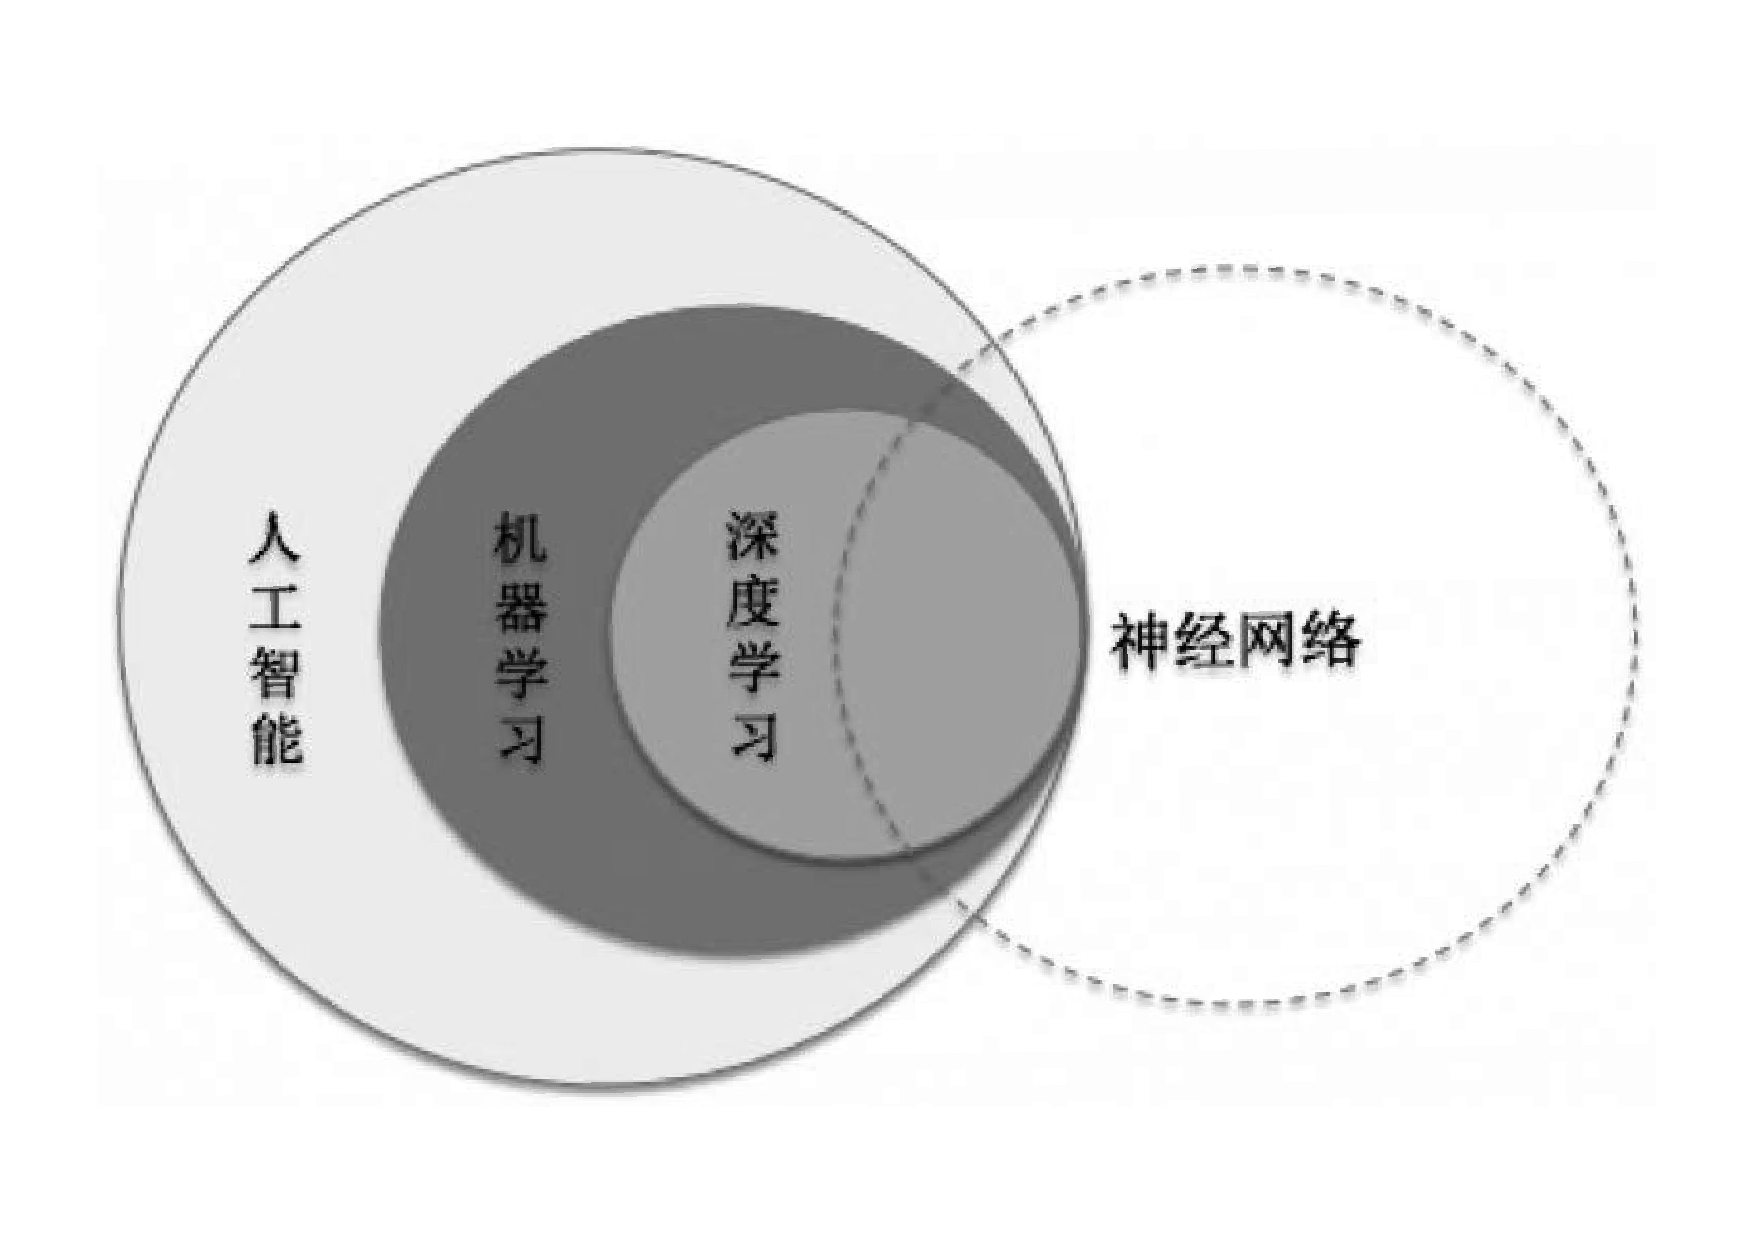
\includegraphics[width=72mm]{Img/chap1_intro/AI_ML.pdf}
  \vspace{-0.6cm}
  \bicaption[人工智能、机器学习、深度学习以及神经网络的逻辑关系]{人工智能、机器学习、深度学习以及神经网络的逻辑关系。}{The relationship between artificial intelligence, machine learning, deep learning and neural network.}
  \label{fig:intro_AI_ML}
\end{figure}

根据目标任务的差异,机器学习分为回归、分类、聚类、异常检测和降维等\citep{gomez2015multimodal,camps2013advances,gislason2006random,muhlbauer2014climatology};根据数据集数据结构的差异,机器学习可以分为空间结构数据学习、序列结构数据学习和时空结构数据学习;根据处理数据种类的差异,机器学习又可分为有监督学习、无监督学习和强化学习等。所谓监督学习,本质上是指数据带有标记(Label),专门用来处理回归和分类问题。机器学习中大多数算法属于监督学习的范畴,比如线性回归(Linear Regression,简称LR)、支持向量回归(Support Vector Regression,简称SVR)、决策树(Decision Tree,简称DT)、随机森林(Random Forest,简称RF)、梯度提升回归(Gradient Boosting Regression Tree,简称GBRT)、极端随机森林回归(Extra Trees Regressor,简称ETR)、K近邻(k-Nearest Neighbor,简称KNN)、卷积神经网络(Convolutional Neural Network,简称CNN)、长短期记忆神经网络(Long Short-Term Memory Recurrent Neural Network,简称LSTM-RNN)等。

很多自然现象可看作是一个复杂系统,例如地震发生机制、板块运动、地下水位变化、太阳活动等,利用现有的经验模型很难精准表达这些系统。减小系统的复杂度(研究个别现象),或加强假设和近似,从可操作且简化的模型中进行推论。但在这两种情况下,难以解释清楚大尺度系统的运行机制。机器学习能自动提取数据的特征,人为因素的干扰大幅度减小,克服了传统经验模型中的许多限制。但机器学习又过度依赖于观测数据,而这些数据难以避免噪声。融合机器学习和物理过程,构建模型,这是目前最有希望也是最具挑战的方法。先进仪器的发展、存储能力的提高、数据量的激增和机器学习理论的发展为模拟这些复杂系统提供了研究途径。本论文基于几种不同的复杂系统,研究了太阳黑子的变化、龙子祠泉流量的动态趋势以及南加州地区中期地震预测。

\section{研究现状、挑战与机遇}\label{sec:intro_veiw}

深度学习兴起前,大多数关于计算机视觉和语音识别等目标任务是基于人工设计的特征和典型的机器学习方法。在计算机视觉领域,常用的人工设计的特征包括SIFT、SURF、HOG、HOF、MBH等。人工设计的特性既是一种优势(对解释性驱动因素的控制),又是一种劣势(过程繁琐,迁移能力差,结果可能是非最优的)。与使用人工设计的特性相比,使用由数据驱动的机器学习有时非常有效。例如,复杂系统涉及到大量的特征,这些特征利用传统意义上的物理模型难以拟合。通常,机器学习在处理复杂任务方面优于物理模型,尤其是在物理机制不完善而观测数据较多时。机器学习可预测某时间段内相对静止的特征,也可用来研究动态变化过程。与半经验性的物理建模方法相比,机器学习少了人工的干预,使用起来更加灵活。在理想的情况下,如果能够完全理解复杂系统的原理,此时没有必要使用机器学习模型。

目前,机器学习的应用领域较为广泛,这里重点关注地球科学领域。地球科学中很多数据集属于时空结构数据,例如大气模拟、海洋运输、火势蔓延、土壤运动、植被碳循环过程等,这些都是时空动力学领域内重要的研究问题\citep{mathieu2015deep,oh2015action};地震波动态时间序列类似于自然语言与信号识别,属于时间结构数据\citep{perol2018convolutional,devries2018deep,rouet2017machine};卫星图像的地形和纹理特征类似于计算机视觉,研究对象通常具有一些描述边缘、纹理、形状和颜色等特征,利用这些特征构建机器学习模型,从而实现对象的定位、分类和检测等目标\citep{lee1990neural}。

尽管机器学习常见的应用领域(计算机视觉和语音识别)与地球科学中的实际问题存在很多的相似之处,但还是有不同的方面。例如,计算机视觉处理的照片有三个通道(红、绿、蓝),高光谱卫星图像会扩展到数百个光谱通道,远远超出可见光范围,这与自然图像的统计特性不同;而且高光谱卫星图像的光谱通道存在空间上的依赖性,违反了数据独立同分布的重要假设;另外,由于地球科学研究中会使用不同的传感器采集不同类型的数据,这些数据存在不同的成像几何、时空分辨率等特征,很难集成这些数据。而且多种类型的传感器收集到的观测数据存在噪声来源不同、数据丢失和系统偏差等问题。

机器学习难以解释时间或空间上的关联性。实际上,在时间或空间中的某一点的过程很容易受到系统状态的影响,这种状态通常隐藏着与时间相关的因素或相邻的网格单元包含相关的系统状态。这种状态难以被观察到,因此特征因子很难被精准地描述。空间和时间高度相关的一个例子是主震和余震的预测,余震的发生不仅取决于瞬时地壳驱动因素,还取决于状态变量,如主震的震级、震区的地质类型等。

一般地,应用机器学习会面临着以下挑战:
\begin{enumerate}
  \item[$\circ$] \textbf{解释能力有待提高}。在解决实际问题时,不仅要考虑提高预测的精度,更要重点关注预测结果的可解释性。目前来说,可解释性是机器学习普遍存在的缺陷\citep{montavon2018methods}。机器学习从观测数据中得到的是统计相关关系,而不是因果关系\citep{runge2015identifying,reichstein2019deep}。为了提高机器学习的可解释性,我们在对数据进行预处理时,需要考虑目标任务可能的因子以及数据集的分布特征。再者,基于神经网络的算法能够给出每个隐藏层的特征值,可视化这些特征值也能在一定程度上观测到模型学到的规则。
  \item[$\circ$] \textbf{增加带标签数据集}。实际应用时并不总是存在带标签的数据集,不仅因为数据集大小的限制,还因为在概念上标记数据存在困难。机器学习中的无监督学习、特征提取、半监督学习等就是针对少数标记的数据\citep{goodfellow2014generative}。
  \item[$\circ$] \textbf{符合自然界普适性的规律}。机器学习通常在训练时性能表现良好,但在外推时结果可能会出现很大的偏差,这可能是由过拟合或观测数据中存在的偏差所致\citep{friedlingstein2014uncertainties}。为达到预期的任务目标,可通过加入普适性的物理规则或提供更丰富的数据。
  \item[$\circ$] \textbf{数据的复杂度}。数据集中包含着复杂的统计学特征、多个任务、噪声来源不同等复杂问题,还要考虑多尺度上的局部关联特征和大范围的全局关联特征。当数据具有较高的复杂度时,可以采取较为复杂的神经网络来挖掘数据信息。
  \item[$\circ$] \textbf{数据具备不确定性}。构建具备不确定性的模型,比如贝叶斯/概率推理方法,从而解决特征之间的因果关系不确定性问题\citep{ghahramani2015probabilistic}。
\end{enumerate}

尽管机器学习在应用过程中存在诸多挑战,但因其强大的信息提取能量,仍旧存在巨大的应用前景。一般地,物理建模和机器学习被看作是两类学科。前者由理论驱动建模,后者由数据驱动建模。在原理方面,物理方法可以解释;在适应数据方面,机器学习具备高度的灵活性,最大化地利用数据的特征能够得到更好的模型和结论。物理建模和机器学习协同作用能够增加模型的可信度\citep{karpatne2017theory,camps2018physics,karpatne2017physics}。从系统建模的角度来看,两者存在以下潜在的协同作用点:
\begin{enumerate}
  \item[$\circ$] \textbf{改进参数的初始化条件}。物理建模需要参数,这些参数难由从初始边界条件得到。机器学习可以自动学习参数。
  \item[$\circ$] \textbf{用机器学习模型替换物理子模型}。如果物理子模型具备半经验性质、功能形式基本存在一定的理论偏差、有足够的观察数据,可考虑结合机器学习和物理子模型,该混合模型结合了物理建模(理论基础、可解释性)和机器学习(数据适应性)的两大优势。这衍生出更具物理性质的机器学习模型,它遵循自然界普适性的定律,调节机制非常灵活,可以从数据中学习。
  \item[$\circ$] \textbf{模型分析与观测不匹配}。假设不存在观测偏差,从观测值中推导出来的物理模型可被视为因知识不完备而导致模型出现了偏差。利用机器学习对结果进行可视化,从而纠正模型的预测。例如,机器学习从数据中提取模式,从而识别物理模型中未显式表达的模式。
\end{enumerate}

\section{论文结构安排}\label{sec:intro_strcture}

论文基于机器学习,利用不同来源的数据集进行处理和分析,发现和理解新知识,推动机器学习的应用。第\ref{chap:ml_theory}章为机器学习理论部分,简要介绍论文涉及到的机器学习的技术原理和方法,然后引出这些模型训练前必要的准备条件。按照数据集的复杂程度,此后几个章节分别研究太阳黑子、泉流量和地震数值预测。针对不同的研究对象设计的具体任务分别进行试验,并对相关的试验结果进行总结与讨论。

第\ref{chap:ml_sunspot}章基于神经网络探测太阳黑子波动情况。太阳黑子是太阳活动的一种表征,太阳活动时刻影响着地球环境和人类经济发展。若能提前预知未来太阳黑子变化趋势,人类能够做出相应的防御措施,进而减小太阳活动带来的损失。从长期记录来看,近几十年来的太阳黑子峰值呈现持续下降的趋势。为了能够时刻跟踪太阳黑子变化,我们采用不同类型的神经网络预测未来1个月、72个月太阳黑子强度。论文中将未来72个月最大的太阳黑子强度视为第25太阳周的峰值。我们重点关注第25太阳周太阳黑子强度。

第\ref{chap:ml_spring}章基于机器学习预测龙子祠泉流量变化。近些年来,人类过度开采地下水,使部分泉水面临干涸的风险,因此合理管理与控制地下水的用量就显得尤为重要。如果能够准确预知未来1个月甚至几个月地下水动态变化的趋势,就能够最大化地利用地下水,从而实现地下水的可持续供应。龙子祠泉具备喀斯特地貌特征,地下水流路径错综复杂,基于半经验的物理模型难以准确预测地下水变化趋势。机器学习擅长处理复杂问题,为预测龙子祠泉的地下水变化提供了研究方法。

第\ref{chap:ml_seismic}章利用机器学习对南加州地区进行中期地震数值预测。原始数据集为1932年至今的南加州地区地震目录。这里选择了中期预报,是因为长期预报需要长时间的数据资料积累(南加州地区地震目录记录最长的年限为$\sim$90年),而短期预报机制更加复杂。基于地震目录得到16个地震因子,其中7个地震因子与空间地震分布密切相关。基于这些地震因子,我们尝试探索未来一年或十年可能发生的最大震级。

第\ref{chap:conclusion}章分别对太阳黑子、泉流量和地震数值预测几个目标任务进行了总结与展望。需要指出的是,论文中很多关于统计学、机器学习中的专业术语并未加以详细区分,比如算法/模型/方法、机器学习/神经网络/深度学习、训练/优化/拟合/模拟/学习等。论文中这些含义近似的术语将会被无差别使用。
